\chapter{Some common finite elements}
\label{element}

\section{Introduction}

There is a jungle of finite elements that have been invented in the early 1940s, and we
will not here give a comprehensive description of the topic. Instead, we will try to motivate
the method by rather simple examples before we discuss some of the general features. 
The formal definition of a finite element~\cite{ciarlet2002finite}: 

\begin{defin}
A finite element is defined by a triplet $(T, V, L)$, where 
\begin{itemize}
\item $T$ is a bounded domain in $\mathbb{R}^d$, most typically a polyhedron; 
\item $V = \{\psi_i\}_{i=1}^n$ is a set of linearly independent basis functions on $T$; 
\item $D = \{d_i\}^n_{i=1}$ is a set of $n$ (linearly independent) 
  degrees of freedom (formally bounded linear functionals on $T$) 
\end{itemize}
\end{defin}
As we see, the term "finite element" refers not only to the cells of the mesh, but also the function space and associated degrees of freedom. The definition is quite abstract, but as we will see, the definition encapsulate precisely what is needed in order to definite a numerical method on a mesh. 

Most commonly, a \emph{nodal basis} is defined as follows 
\begin{defin}
\label{nodal:basis}
The nodal basis for the triplet  $(T, V, L)$ is defined as the set of basis functions
$\{\phi_i\}^n_{i=1}$ that satisfies  
\[
d_j(\phi_i) = \delta_{ij}, \quad for 1 \le i,j \le n. 
\]
The $\{d_j\}^n_{i=1}$ is often called the dual basis of the finite element.  
\end{defin}

\section{Some example finite elements: Lagrange and Hermite on the unit interval. }
Let us now try to make this concrete in a couple of simple examples. First we notie that  
in the above, we have two function spaces $\{\psi_i\}$ and $\{\phi_i\}$. Clearly, 
\[
\phi_i = \sum \alpha_{ij}\psi_j,  
\]
where the matrix $\alpha_{ij}$ is determined such that 
\[
d_i(\phi_j) = \delta_{ij}. 
\]
Hence, let then $V=\mathbb{P}_k$ and lets consider the Lagrange and Hermite elements, defined in terms
of Lagrange and Hermite interpolation, respectively.  
On the unit interval
\[
\mathbb{P}_k = \{1, x, \ldots, x^k\}. 
\]
Clearly, $\mathbb{P}_k$ has $k+1$ basis functions  and they are all linearly independent. 
The Lagrange and Hermite elements are then defined in the examples below. 
\begin{exmp}[\textbf{The Lagrange element in 1D.}]
\label{lagrange:element}
Lagrange interpolation is defined simply by nodal values in a set of points. Hence, 
let 
\[
x_j = j \Delta x, \quad \Delta x = \frac{1}{k}, \quad  j= 0, \dots, k 
\]
Then the j'th Lagrange function $L_j$ can be written as a linear combination the basis of $\mathbb{P}_k$ as 
\[ 
L_j = \sum_i \alpha_{ij} x^i 
\]
where $\alpha_{ij}$ are determined by 
\[ 
d_i(L_j) = L_j(x_i) = \delta_{ij} . 
\]
In 1D, an explicit formulation can be derived for $L_j$, namely 
\[
L_j(x) = \frac{x-x_0}{x_j-x_0} \ldots \frac{x-x_{j-1}}{x_j-x_{j-1}} \ldots \frac{x-x_{j+1}}{x_j-x_{j+1}} \ldots \frac{x-x_k}{x_j-x_k}  
\]
Clearly, for instance $L_j(x_0) = 0$ whereas  $L_j(x_j) = 1$.  
\end{exmp}
Calculating the basis for a Lagrange element yields and explicit formula in 1D, but is harder in higher dimensions.
The following code computes the basis directly from the abstract definition without references to the above formula, using SymPy.  
\begin{python}
from sympy import * 

def dirac(i,j): 
  if i == j: return 1 
  else: return 0 

k = 5  
x = Symbol("x") 
dx = 1/k 

basis = [x**j for j in range(0, k+1)] 
points = [j*dx for j in range(0, k+1)] 
dofs = symbols("a:%d"%(k+1))

print ("A basis for the polynomial space ", basis) 
print ("A set of points to use for computing the nodal basis ", points) 
print ("The degrees of freedom, represented as symbols ", dofs) 

pol = sum([dofs[i]*basis[i] for i in range(0, (k+1))])   
print ("A generic function is then ", pol)

Lagrange_basis = []
for i in range(0, (k+1)): 
  equations = []
  for j in range(len(points)):  
    p = points[j]
    eq = pol.subs(x,p) - dirac(i,j) 
    equations.append(eq)
  coeff = solve(equations, dofs) 
  Nj = pol.subs(coeff)
  Lagrange_basis.append(Nj) 

print (Lagrange_basis) 

# check that the Lagrange basis is what it is supposed to be 
for i, basis in enumerate(Lagrange_basis): 
    for j, point in enumerate(points): 
        print ("i,j ", i,j, " basis evaluation ",  "%0.3f" % basis.subs({ x: point})) 
\end{python}
The output is as follows: 
\begin{python}
A basis for the polynomial space  [1, x, x**2, x**3, x**4, x**5]
A set of points to use for computing the nodal basis  [0.0, 0.2, 0.4, 0.6000000000000001, 0.8, 1.0]
The degrees of freedom, represented as symbols  (a0, a1, a2, a3, a4, a5)
A generic function is then  a0 + a1*x + a2*x**2 + a3*x**3 + a4*x**4 + a5*x**5
[-26.0416666666667*x**5 + 78.125*x**4 - 88.5416666666667*x**3 + 46.875*x**2 - 11.4166666666667*x + 1.0, ....]
i,j  0 0  basis evaluation  1.000
i,j  0 1  basis evaluation  0.000
...
\end{python}
The 6 basis functions of the Largrange element of order 5 is shown in Fig. \ref{fig:Lagrange5}. 
Exercise \ref{lagrange:triangle} will consider a code for defining a Lagrange element of arbitrary order on a reference triangle.  

\begin{figure}
\begin{center}
\includegraphics[width=0.75\textwidth]{chapters/element/plots/Lagrange5.png}
\caption{
The basis function of the Lagrange element of order 5. }
\label{fig:Lagrange5}
\end{center}
\end{figure}


The Hermite interpolation generalize the Lagrange interpolation by including also derivative. As such 
the Hermite element is defined in terms of the Hermite interpolation. This is detailed in the following example: 
\begin{exmp}{\textbf{The Hermite element in 1D}.} 
\label{hermite:element}
Let us consider the Hermite interpolation onto $k+1$ points.  
Each point is associated with two degrees of freedom, the function evaluation and the evaluation of the first 
derivative of the function.  
using $m$ derivatives in each point.Hence,  
the number of degrees of freedom, or the number of equations defined by the specification of the nodal 
basis in Definition \ref{nodal:basis} are then $2(k+1)$. As such our polynomial space would be $\mathbb{P}_{2(k+1)}$.    
As such, we may once again compute the nodal basis of the Hermite element. 
Let $H_j$ be the j'th nodal basis, expressed as  
\[ 
H_j = \sum_i \alpha_{ij} x^i 
\]
Then 
where $\alpha_{ij}$ are determined by 
\[ 
d_i(L_j) = L_j(x_i) = \delta_{ij} . 
\]
Here, lets split the degrees of freedom into even and odd numbers, where the even numbering refers to 
point evaluations whereas the odd numbers are the evaluation of the derivatives. 
That is 
\begin{align*} 
d_i(H_j) &= H_j(x_i)  &=  \delta_{ij}, \quad \mbox{ even } i,j   \\
d_i(H_j) &= H'_j(x) |_{x=x_i} &= \delta_{ij}, \quad \mbox{ odd } i,j  
\end{align*}

\end{exmp}

There are a couple of observations that makes the above definite of the finite element really useful 1)   
the mapping between an arbitrary cell of a general mesh and the reference cell can be generalized to 
a mapping between an arbitrary finite element on the mesh and a corresponding reference element and 2)
the degrees of freedom implicitly defines the connectivety of the finite elements in terms of the
connectivity of the underlying cells of the mesh. These observations are detailed below.    

\section{Mapping a reference element onto a physical element. }
Let $x$ and $\hat{x}$ be coordiates in the domains $T$ and $\hat{T}$, respectively, and  
for simplicity we assume an affine mapping between the coordinates:  
\[
x = F_T(\hat{x}) = A_T \hat{x} + x_0   
\]
The Jacobian of the mapping is 
\[
\frac{\partial x}{\partial \hat{x}} = J(\hat{x}) = A_T      
\]
For isoparametric elements, a basis function $\phi$
is the simply defined in terms of its associated function $\hat{\phi}$
on the reference
element, ie. 
\[
\phi(x) = \hat{\phi}(\hat{x}) .  
\]
With this definition we may easily evaluate integrals
\[
\int_T \phi(x) dx = \int_{\hat{T}} \hat{\phi}(\hat{x}) det J d\hat{x},  
\]
and derivatives 
\[
\frac{\partial \phi}{\partial x_i } = \sum_j  \frac{\partial \hat{\phi}}{\partial \hat{x}_j } \frac{\partial \hat{x}_j}{\partial \hat{x}_i } 
\]
As such the finite element engines may perform all the computations on the reference cells, which makes the implementation easy and efficient. 

\section{The connectivity of the mesh and the corresponding finite element space}

The Lagrange element of order 5 was illustrated in Fig.~\cite{fig:Lagrange}. We observe here that the basis function $0$ and $5$ are associated
with the edges $x=0$ and $x=1$, whereas the other functions are all zero at the edges. Hence, the basis function $1, \ldots, 4$ do not connect 
to any other element, whereas the basis $0$ would directly connect to the a corresponding element on the left whereas basis $5$ connects to the 
an element on the right, if present. Hence the edge nodes defines the connectivity and hereby the continuity towards the neighbouring elements. 



\begin{figure}
\begin{center}
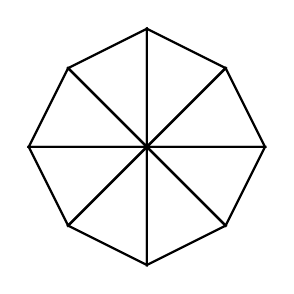
\begin{tikzpicture}
\draw[black, thick] (0,0) -- (1,1) -- (0,1.5) -- cycle;
\draw[black, thick] (0,0) -- (1,1) -- (1.5,0) -- cycle;
\draw[black, thick] (0,0) -- (1,-1) -- (1.5,0) -- cycle;
\draw[black, thick] (0,0) -- (1,-1) -- (0,-1.5) -- cycle;
\draw[black, thick] (0,0) -- (-1,-1) -- (-1.5,0) -- cycle;
\draw[black, thick] (0,0) -- (-1,-1) -- (0,-1.5) -- cycle;
\draw[black, thick] (0,0) -- (-1,1) -- (0,1.5) -- cycle;
\draw[black, thick] (0,0) -- (-1,1) -- (-1.5,0) -- cycle;
\end{tikzpicture}
\caption{
A simple mesh with 8 triangles all meeting at a common point.}
\label{fig:Lagrange5}
\end{center}
\end{figure}




\section{Exercises}
\begin{exercise}
\label{hermite:interval}
Make a Python code that defines a Hermite on the unit interval.       
\end{exercise}



\begin{exercise}
\label{lagrange:triangle}
Make a Python code that defines a Lagrange element of arbitrary order on the reference triangle 
consisting of the vertices $(0,0)$, $(1,0)$ and $(0,1)$. Let $\mathbb{P}_k = \{ x^i y^j \} \mbox{ for } i,j \mbox{ such that } i+j \le k\} $     
\end{exercise}

\begin{exercise}
Check that the interpolation result
of the Bramble-Hilbert lemma \ref{bramblehilbert} applies to the Lagrange interpolation on the unit line. Consider 
for example a function $f = sin(x)$ on the unit interval. The function $f$ is a good example as it cannot be expressed 
as a polynomial of finite order, but can be approximated arbitrary well. 
\end{exercise}

\begin{exercise}
Compute the condition number of the mass matrix when using the Lagrange and the Hermite basis. Compare it with the condition
number when using the basis consisting of monomials, ie. $(1, x, x^2, \ldots)$.   
	The mass matrix on the unit interval  is the matrix $M_{ij} = \int_0^1 \phi_i \phi_j \, dx $ where $\{\phi_i\}$ is 
	the set of basis functions in use. 
\end{exercise}





